%%
%% Automatically generated file from DocOnce source
%% (https://github.com/doconce/doconce/)
%%
% #define PREAMBLE
% #ifdef PREAMBLE
%-------------------- begin preamble ----------------------
\documentclass[%
oneside,                 % oneside: electronic viewing, twoside: printing
final,                   % draft: marks overfull hboxes, figures with paths
10pt]{article}
\listfiles               %  print all files needed to compile this document
\usepackage{relsize,makeidx,color,setspace,amsmath,amsfonts,amssymb}
\usepackage[table]{xcolor}
\usepackage{bm,ltablex,microtype}
\usepackage[pdftex]{graphicx}
\usepackage{fancybox}  % make sure fancybox is loaded before fancyvrb
%\setlength{\fboxsep}{8pt}  % may clash with need in pre/cod envirs
% Packages for typesetting blocks of computer code
\usepackage{fancyvrb,framed,moreverb}
% Define colors
\definecolor{orange}{cmyk}{0,0.4,0.8,0.2}
\definecolor{tucorange}{rgb}{1.0,0.64,0}
\definecolor{darkorange}{rgb}{.71,0.21,0.01}
\definecolor{darkgreen}{rgb}{.12,.54,.11}
\definecolor{myteal}{rgb}{.26, .44, .56}
\definecolor{gray}{gray}{0.45}
\definecolor{mediumgray}{gray}{.8}
\definecolor{lightgray}{gray}{.95}
\definecolor{brown}{rgb}{0.54,0.27,0.07}
\definecolor{purple}{rgb}{0.5,0.0,0.5}
\definecolor{darkgray}{gray}{0.25}
\definecolor{darkblue}{rgb}{0,0.08,0.45}
\definecolor{darkblue2}{rgb}{0,0,0.8}
\definecolor{lightred}{rgb}{1.0,0.39,0.28}
\definecolor{lightgreen}{rgb}{0.48,0.99,0.0}
\definecolor{lightblue}{rgb}{0.53,0.81,0.92}
\definecolor{lightblue2}{rgb}{0.3,0.3,1.0}
\definecolor{lightpurple}{rgb}{0.87,0.63,0.87}
\definecolor{lightcyan}{rgb}{0.5,1.0,0.83}
\colorlet{comment_green}{green!50!black}
\colorlet{string_red}{red!60!black}
\colorlet{keyword_pink}{magenta!70!black}
\colorlet{indendifier_green}{green!70!white}
% Backgrounds for code
\definecolor{cbg_gray}{rgb}{.95, .95, .95}
\definecolor{bar_gray}{rgb}{.92, .92, .92}
\definecolor{cbg_yellowgray}{rgb}{.95, .95, .85}
\definecolor{bar_yellowgray}{rgb}{.95, .95, .65}
\colorlet{cbg_yellow2}{yellow!10}
\colorlet{bar_yellow2}{yellow!20}
\definecolor{cbg_yellow1}{rgb}{.98, .98, 0.8}
\definecolor{bar_yellow1}{rgb}{.98, .98, 0.4}
\definecolor{cbg_red1}{rgb}{1, 0.85, 0.85}
\definecolor{bar_red1}{rgb}{1, 0.75, 0.85}
\definecolor{cbg_blue1}{rgb}{0.87843, 0.95686, 1.0}
\definecolor{bar_blue1}{rgb}{0.7,     0.95686, 1}
\usepackage{listingsutf8}
% Common lstlisting parameters
\usepackage{calc}
\newlength{\lstboxwidth}  % width of lst box
\newlength{\framethickness}
\setlength{\framethickness}{0.5mm}
% for frame=trbl and a framerule that has significant size, set
% xleftmargin=5mm and xrightmargin=5mm.
\lstset{
  basicstyle=\small \ttfamily,
  breaklines=false,          % break/wrap lines
  breakatwhitespace=true,    % let linebreaks happen at whitespace
  breakindent=40pt,
  tab=,
  tabsize=4,                 % tab means 4 spaces
  %belowskip=\smallskipamount,  % space between code and text below
  xleftmargin=2mm,           % indentation of code frame
  xrightmargin=0mm,
  framexleftmargin=2mm,      % add frame space to the left of the code box
  %numbers=left,             % put line numbers on the left
  %stepnumber=2,             % stepnumber=1 numbers each line, =n every n lines
  framerule=\framethickness, % thickness of frame
  aboveskip=2ex,             % vertical space above code frame
  showstringspaces=false,    % show spaces in strings with an underscore
  showspaces=false,          % show spaces with an underscore
  showtabs=false,
  keepspaces=true,
  columns=fullflexible,      % tighter character kerning, like verb
  escapeinside={(*@}{@*)},   % (*@ \pause @*) in slides and math in code blocks
  extendedchars=\true,       % allows non-ascii chars, does not work with utf-8
}
% Internally defined styles for lstlisting
\lstdefinestyle{simple}{
commentstyle={},
}
% end of custom lstdefinestyles
\usepackage[T1]{fontenc}
%\usepackage[latin1]{inputenc}
\usepackage{ucs}
\usepackage[utf8x]{inputenc}
\usepackage{lmodern}         % Latin Modern fonts derived from Computer Modern
% Hyperlinks in PDF:
\definecolor{linkcolor}{rgb}{0,0,0.4}
\usepackage{hyperref}
\hypersetup{
    breaklinks=true,
    colorlinks=true,
    linkcolor=linkcolor,
    urlcolor=linkcolor,
    citecolor=black,
    filecolor=black,
    %filecolor=blue,
    pdfmenubar=true,
    pdftoolbar=true,
    bookmarksdepth=3   % Uncomment (and tweak) for PDF bookmarks with more levels than the TOC
    }
%\hyperbaseurl{}   % hyperlinks are relative to this root
\setcounter{tocdepth}{2}  % levels in table of contents
% Tricks for having figures close to where they are defined:
% 1. define less restrictive rules for where to put figures
\setcounter{topnumber}{2}
\setcounter{bottomnumber}{2}
\setcounter{totalnumber}{4}
\renewcommand{\topfraction}{0.95}
\renewcommand{\bottomfraction}{0.95}
\renewcommand{\textfraction}{0}
\renewcommand{\floatpagefraction}{0.75}
% floatpagefraction must always be less than topfraction!
% 2. ensure all figures are flushed before next section
\usepackage[section]{placeins}
% 3. enable begin{figure}[H] (often leads to ugly pagebreaks)
%\usepackage{float}\restylefloat{figure}
% --- fancyhdr package for fancy headers ---
\usepackage{fancyhdr}
\fancyhf{} % sets both header and footer to nothing
\renewcommand{\headrulewidth}{0pt}
\fancyfoot[LE,RO]{\thepage}
% Ensure copyright on titlepage (article style) and chapter pages (book style)
\fancypagestyle{plain}{
  \fancyhf{}
  \fancyfoot[C]{{\footnotesize \copyright\ 2021, H. P. Langtangen. Made with \href{https://github.com/doconce/doconce}{DocOnce}}}
%  \renewcommand{\footrulewidth}{0mm}
  \renewcommand{\headrulewidth}{0mm}
}
% Ensure copyright on titlepages with \thispagestyle{empty}
\fancypagestyle{empty}{
  \fancyhf{}
  \fancyfoot[C]{{\footnotesize \copyright\ 2021, H. P. Langtangen. Made with \href{https://github.com/doconce/doconce}{DocOnce}}}
  \renewcommand{\footrulewidth}{0mm}
  \renewcommand{\headrulewidth}{0mm}
}
\pagestyle{fancy}
\usepackage[framemethod=TikZ]{mdframed}
% --- begin definitions of admonition environments ---
% Admonition style "mdfbox" is an oval colored box based on mdframed
% "notice" admon
\colorlet{mdfbox_notice_background}{darkgray!20!white}
\newmdenv[
  skipabove=15pt,
  skipbelow=15pt,
  outerlinewidth=0,
  backgroundcolor=mdfbox_notice_background,
  linecolor=black,
  linewidth=2pt,       % frame thickness
  frametitlebackgroundcolor=darkgray!40!white,
  frametitlerule=true,
  frametitlefont=\normalfont\bfseries,
  shadow=false,        % frame shadow?
  shadowsize=11pt,
  leftmargin=0,
  rightmargin=0,
  roundcorner=5,
  needspace=0pt,
]{notice_mdfboxmdframed}
\newenvironment{notice_mdfboxadmon}[1][]{
\begin{notice_mdfboxmdframed}[frametitle=#1]
}
{
\end{notice_mdfboxmdframed}
}
% Admonition style "mdfbox" is an oval colored box based on mdframed
% "summary" admon
\colorlet{mdfbox_summary_background}{tucorange!20!white}
\newmdenv[
  skipabove=15pt,
  skipbelow=15pt,
  outerlinewidth=0,
  backgroundcolor=mdfbox_summary_background,
  linecolor=black,
  linewidth=2pt,       % frame thickness
  frametitlebackgroundcolor=tucorange!40!white,
  frametitlerule=true,
  frametitlefont=\normalfont\bfseries,
  shadow=false,        % frame shadow?
  shadowsize=11pt,
  leftmargin=0,
  rightmargin=0,
  roundcorner=5,
  needspace=0pt,
]{summary_mdfboxmdframed}
\newenvironment{summary_mdfboxadmon}[1][]{
\begin{summary_mdfboxmdframed}[frametitle=#1]
}
{
\end{summary_mdfboxmdframed}
}
% Admonition style "mdfbox" is an oval colored box based on mdframed
% "warning" admon
\colorlet{mdfbox_warning_background}{darkgreen!40!white}
\newmdenv[
  skipabove=15pt,
  skipbelow=15pt,
  outerlinewidth=0,
  backgroundcolor=mdfbox_warning_background,
  linecolor=black,
  linewidth=2pt,       % frame thickness
  frametitlebackgroundcolor=darkgreen!80!white,
  frametitlerule=true,
  frametitlefont=\normalfont\bfseries,
  shadow=false,        % frame shadow?
  shadowsize=11pt,
  leftmargin=0,
  rightmargin=0,
  roundcorner=5,
  needspace=0pt,
]{warning_mdfboxmdframed}
\newenvironment{warning_mdfboxadmon}[1][]{
\begin{warning_mdfboxmdframed}[frametitle=#1]
}
{
\end{warning_mdfboxmdframed}
}
% Admonition style "mdfbox" is an oval colored box based on mdframed
% "question" admon
\colorlet{mdfbox_question_background}{red!50!white}
\newmdenv[
  skipabove=15pt,
  skipbelow=15pt,
  outerlinewidth=0,
  backgroundcolor=mdfbox_question_background,
  linecolor=black,
  linewidth=2pt,       % frame thickness
  frametitlebackgroundcolor=red!90!white,
  frametitlerule=true,
  frametitlefont=\normalfont\bfseries,
  shadow=false,        % frame shadow?
  shadowsize=11pt,
  leftmargin=0,
  rightmargin=0,
  roundcorner=5,
  needspace=0pt,
]{question_mdfboxmdframed}
\newenvironment{question_mdfboxadmon}[1][]{
\begin{question_mdfboxmdframed}[frametitle=#1]
}
{
\end{question_mdfboxmdframed}
}
% Admonition style "mdfbox" is an oval colored box based on mdframed
% "block" admon
\colorlet{mdfbox_block_background}{darkgreen!40!white}
\newmdenv[
  skipabove=15pt,
  skipbelow=15pt,
  outerlinewidth=0,
  backgroundcolor=mdfbox_block_background,
  linecolor=black,
  linewidth=2pt,       % frame thickness
  frametitlebackgroundcolor=darkgreen!80!white,
  frametitlerule=true,
  frametitlefont=\normalfont\bfseries,
  shadow=false,        % frame shadow?
  shadowsize=11pt,
  leftmargin=0,
  rightmargin=0,
  roundcorner=5,
  needspace=0pt,
]{block_mdfboxmdframed}
\newenvironment{block_mdfboxadmon}[1][]{
\begin{block_mdfboxmdframed}[frametitle=#1]
}
{
\end{block_mdfboxmdframed}
}
% --- end of definitions of admonition environments ---
% prevent orhpans and widows
\clubpenalty = 10000
\widowpenalty = 10000
% --- end of standard preamble for documents ---
% insert custom LaTeX commands...
\raggedbottom
\makeindex
\usepackage[totoc]{idxlayout}   % for index in the toc
\usepackage[nottoc]{tocbibind}  % for references/bibliography in the toc
%-------------------- end preamble ----------------------
\begin{document}
% matching end for #ifdef PREAMBLE
% #endif
\newcommand{\exercisesection}[1]{\subsection*{#1}}
\input{newcommands_bfmath}
\input{newcommands_replace}
% ------------------- main content ----------------------
% ----------------- title -------------------------
\thispagestyle{empty}
\begin{center}
{\LARGE\bf
\begin{spacing}{1.25}
Testing admons
\end{spacing}
}
\end{center}
% ----------------- author(s) -------------------------
\begin{center}
{\bf H. P. Langtangen${}^{}$} \\ [0mm]
\end{center}
\begin{center}
% List of all institutions:
\end{center}
    
% ----------------- end author(s) -------------------------
% --- begin date ---
\begin{center}
Jan 32, 2100
\end{center}
% --- end date ---
\vspace{1cm}
% !split
\section{Introduction}
First some ordinary text to compare font sizes in admonitions
and the surrounding text.
\subsection{Code}
Need some code outside admons for color and font comparisons:
\begin{lstlisting}[language=Python,style=simple,xleftmargin=2mm]
def some_code(x):
    return sin(x)*exp(1-x)

\end{lstlisting}

And some plain text verbatim:
\begin{lstlisting}[language=Python,style=simple,xleftmargin=2mm]
x=1.0 y=0.9 z=0.4
x=1.1 y=0.3 z=0.1

\end{lstlisting}

\subsection{Quotes and boxes}
Here is a plain quote environment.

\begin{quote}
Sayre's law states that
``in any dispute the intensity of feeling is inversely
proportional to the value of the issues at stake.'' \\
By way of corollary, it adds: \\
``That is why academic politics are so bitter.'' \\
\emph{Source}: \href{{https://en.wikipedia.org/wiki/Sayre's_law}}{wikipedia}
\end{quote}

Does quotes with title also work? No...cannot work in {\LaTeX} and HTML
and then it does not make sense to support it.
A plain \emph{box} is sometimes useful. Let's show it here for comparison
with admons (especially the block admon has much in common with a box).
The box is more aimed at framing a law or an equation.
First a simple block with text, an equation, and a list:

\begin{center}
\begin{Sbox}
\begin{minipage}{0.85\linewidth}
A generic equation
\[ f(x) = 0 \]
must be solved by a numerical method, such as
\begin{itemize}
 \item Newton's method
 \item The Bisection method
 \item Fixed-point (Picard) iteration by rewriting $f(x)=x - g(x)$
 \item The Secant method
\end{itemize}
\noindent
\end{minipage}
\end{Sbox}
\fbox{\TheSbox}
\end{center}
Now test a box with equation only (note that this line continues the
box, it is not a new paragraph):

\begin{center}
\begin{Sbox}
\begin{minipage}{0.85\linewidth}
\begin{equation} f(x) = \sin(x)e^{1-x} \end{equation}
\end{minipage}
\end{Sbox}
\fbox{\TheSbox}
\end{center}
\paragraph{Hint.}
Newton's method requires a good start vector to converge fast.


Let's begin a new paragraph and show a box with code only:

\begin{center}
\begin{Sbox}
\begin{minipage}{0.85\linewidth}
\begin{lstlisting}[language=Python,style=simple,xleftmargin=2mm]
def some_code(x):
    return sin(x)*exp(1-x)

\end{lstlisting}
\end{minipage}
\end{Sbox}
\fbox{\TheSbox}
\end{center}
\subsection{Admonitions}
Let us start with a plain warning environment.

\begin{warning_mdfboxadmon}[Warning.]
And here is a warning about something to pay attention to. We
test how the heading behave and add quite some extra texts
in comparison with the other admons.
\begin{itemize}
  \item and a list
  \item with items
\end{itemize}
\noindent
We continue with more text to see how that affects the layout.
And more and more text.
And more and more text.
And more and more text.
And more and more text.
And more and more text.
And more and more text.
\end{warning_mdfboxadmon} % title: Warning.


Test warning with title:

\begin{warning_mdfboxadmon}[{\large Title ending with math $\sqrt{2}\approx 1.4$}.]
{\large And here comes some text with bad news in larger font.
Also some code:
\begin{lstlisting}[language=Python,style=simple,xleftmargin=2mm]
def f(x):
    return x

\end{lstlisting}

And a complete program
\begin{lstlisting}[language=Python,style=simple,xleftmargin=2mm]
print("Hello, World!")

\end{lstlisting}
\par}
\end{warning_mdfboxadmon} % title: {\large Title ending with math $\sqrt{2}\approx 1.4$}.


Test warning with large title with math:

\begin{warning_mdfboxadmon}[{\large Watch out for $\nabla\cdot\bm{u}=0$ equations}.]
{\large Divergence freedom is often problematic from a numerical point
of view.
\par}
\end{warning_mdfboxadmon} % title: {\large Watch out for $\nabla\cdot\bm{u}=0$ equations}.


Then we test a block, which is guaranteed to never have any admon icon.

\begin{block_mdfboxadmon}[Block with title.]
\vspace{0.5mm}\par\noindent
{\footnotesize Here is a block of text with title. It is typeset
\emph{without any icon} and is useful when you want some admons with icon
and some without. With the small font size, as used here, one can have
more comment-style text or text that really goes deeper or talks
about fun facts that are not strictly necessary for the main flow
of understanding.
\par}
\end{block_mdfboxadmon} % title: Block with title.



\begin{block_mdfboxadmon}[]
Here is a block of text with no title. As above, it is typeset without any icon
and is useful when you want some admons with icon and some without.
\end{block_mdfboxadmon} % title: 


% Note that the final ! does not appear in Sphinx and reST since
% those formats automatically add : to the admonition title.

\begin{notice_mdfboxadmon}[Note eventually!]
Ah, we are soon close to the end (with illegal font size specification!).
But first a bit of math where we define $\theta$ and $\bm{r}$:
\begin{align*}
\theta &= q^2,\\
\bm{r} &= \varrho\bm{i}
\end{align*}
\end{notice_mdfboxadmon} % title: Note eventually!


% Test one word with a number

\begin{notice_mdfboxadmon}[Point1.]
Ah, we are soon close to the end.
\end{notice_mdfboxadmon} % title: Point1.



\begin{question_mdfboxadmon}[Question.]
So, how many admonition environments does DocOnce support?
\end{question_mdfboxadmon} % title: Question.



\begin{question_mdfboxadmon}[Question.]
\begin{enumerate}
 \item Once more, how many admonition environments does DocOnce support?
\end{enumerate}
\noindent
\end{question_mdfboxadmon} % title: Question.



\begin{warning_mdfboxadmon}[Tip.]
It is of outmost important to
\begin{enumerate}
\item stay cool
\item read hints and tips carefully
\end{enumerate}
\noindent
Because here the thing is to do
\begin{lstlisting}[language=Python,style=simple,xleftmargin=2mm]
import urllib

def grab(url, filename):
    urllib.urlretrieve(url, filename=filename)

\end{lstlisting}
\end{warning_mdfboxadmon} % title: Tip.


Next is a warning without a title ("none" implies no title).

\begin{warning_mdfboxadmon}[]
And here comes some text with bad news.
\end{warning_mdfboxadmon} % title: 


\subsection{Going deeper environments}
Here is a long notice environment with a custom title and much
text, math and code.

\begin{notice_mdfboxadmon}[Going deeper.]
We have some equations that should be preceded by much text, so the
task is to write and write. The number of words, and not the
meaning, is what counts here. We need desperately to fill up the
page in the hope that some admonitions will experience a page break,
which the {\LaTeX} environment should handle with ease.
Let us start with some equations:
\begin{align*}
\Ddt{u} &= 0
\\
\half &= \halfi\\
\half\x &= \normalvec
\end{align*}
The implementation of such complicated equations in computer
code is task that this "Going deeper" environment targets.
\begin{lstlisting}[language=Python,style=simple,xleftmargin=2mm]
def Dudt(u):
    r = diff(u, t) + u*grad(u)
    return r

half = 0.5
x = 2*n

\end{lstlisting}

And some more text that can help going into the next page.
Longer computer code requires vertical space:
\begin{lstlisting}[language=Python,style=simple,xleftmargin=2mm]
class Diff:
    def __init__(self, f, h=1E-5):
        self.f = f
        self.h = float(h)

class Forward1(Diff):
    def __call__(self, x):
        f, h = self.f, self.h
        return (f(x+h) - f(x))/h

class Backward1(Diff):
    def __call__(self, x):
        f, h = self.f, self.h
        return (f(x) - f(x-h))/h

class Central2(Diff):
    def __call__(self, x):
        f, h = self.f, self.h
        return (f(x+h) - f(x-h))/(2*h)

class Central4(Diff):
    def __call__(self, x):
        f, h = self.f, self.h
        return (4./3)*(f(x+h)   - f(x-h))  /(2*h) - \
               (1./3)*(f(x+2*h) - f(x-2*h))/(4*h)

class Central6(Diff):
    def __call__(self, x):
        f, h = self.f, self.h
        return (3./2) *(f(x+h)   - f(x-h))  /(2*h) - \
               (3./5) *(f(x+2*h) - f(x-2*h))/(4*h) + \
               (1./10)*(f(x+3*h) - f(x-3*h))/(6*h)

class Forward3(Diff):
    def __call__(self, x):
        f, h = self.f, self.h
        return (-(1./6)*f(x+2*h) + f(x+h) - 0.5*f(x) - \
                (1./3)*f(x-h))/h

\end{lstlisting}

And then we add a figure too.
\vspace{6mm}
% inline figure
\centerline{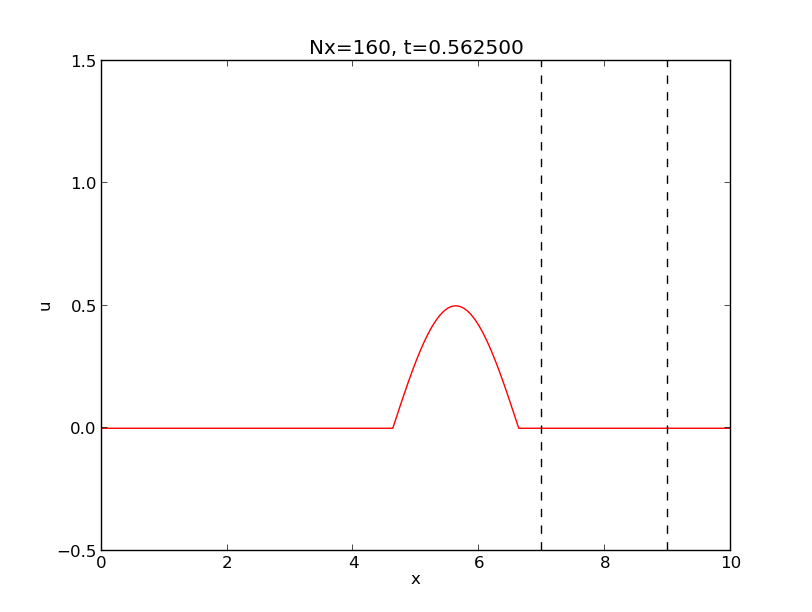
\includegraphics[width=0.7\linewidth]{testfigs/wave1D.png}}
\vspace{6mm}
\end{notice_mdfboxadmon} % title: Going deeper.


\subsection{The end}
A bit of text before the summary, which we now call "Concluding remarks,
for the novice",
just because we can.

\begin{summary_mdfboxadmon}[Concluding remarks for the novice.]
We can summarize the most important things with admons: they have
a different typesetting, and they may have a symbol.
Titles should be optional.
\end{summary_mdfboxadmon} % title: Concluding remarks for the novice.


\paragraph{Remark.}
The \texttt{remarks} and \texttt{hint} environments are not allowed outside
exercises (and problems and projects too).
% ------------------- end of main content ---------------
% #ifdef PREAMBLE
\end{document}
% #endif

